% Options for packages loaded elsewhere
% Options for packages loaded elsewhere
\PassOptionsToPackage{unicode}{hyperref}
\PassOptionsToPackage{hyphens}{url}
\PassOptionsToPackage{dvipsnames,svgnames,x11names}{xcolor}
%
\documentclass[
  letterpaper,
  DIV=11,
  numbers=noendperiod]{scrreprt}
\usepackage{xcolor}
\usepackage{amsmath,amssymb}
\setcounter{secnumdepth}{5}
\usepackage{iftex}
\ifPDFTeX
  \usepackage[T1]{fontenc}
  \usepackage[utf8]{inputenc}
  \usepackage{textcomp} % provide euro and other symbols
\else % if luatex or xetex
  \usepackage{unicode-math} % this also loads fontspec
  \defaultfontfeatures{Scale=MatchLowercase}
  \defaultfontfeatures[\rmfamily]{Ligatures=TeX,Scale=1}
\fi
\usepackage{lmodern}
\ifPDFTeX\else
  % xetex/luatex font selection
\fi
% Use upquote if available, for straight quotes in verbatim environments
\IfFileExists{upquote.sty}{\usepackage{upquote}}{}
\IfFileExists{microtype.sty}{% use microtype if available
  \usepackage[]{microtype}
  \UseMicrotypeSet[protrusion]{basicmath} % disable protrusion for tt fonts
}{}
\makeatletter
\@ifundefined{KOMAClassName}{% if non-KOMA class
  \IfFileExists{parskip.sty}{%
    \usepackage{parskip}
  }{% else
    \setlength{\parindent}{0pt}
    \setlength{\parskip}{6pt plus 2pt minus 1pt}}
}{% if KOMA class
  \KOMAoptions{parskip=half}}
\makeatother
% Make \paragraph and \subparagraph free-standing
\makeatletter
\ifx\paragraph\undefined\else
  \let\oldparagraph\paragraph
  \renewcommand{\paragraph}{
    \@ifstar
      \xxxParagraphStar
      \xxxParagraphNoStar
  }
  \newcommand{\xxxParagraphStar}[1]{\oldparagraph*{#1}\mbox{}}
  \newcommand{\xxxParagraphNoStar}[1]{\oldparagraph{#1}\mbox{}}
\fi
\ifx\subparagraph\undefined\else
  \let\oldsubparagraph\subparagraph
  \renewcommand{\subparagraph}{
    \@ifstar
      \xxxSubParagraphStar
      \xxxSubParagraphNoStar
  }
  \newcommand{\xxxSubParagraphStar}[1]{\oldsubparagraph*{#1}\mbox{}}
  \newcommand{\xxxSubParagraphNoStar}[1]{\oldsubparagraph{#1}\mbox{}}
\fi
\makeatother


\usepackage{longtable,booktabs,array}
\usepackage{calc} % for calculating minipage widths
% Correct order of tables after \paragraph or \subparagraph
\usepackage{etoolbox}
\makeatletter
\patchcmd\longtable{\par}{\if@noskipsec\mbox{}\fi\par}{}{}
\makeatother
% Allow footnotes in longtable head/foot
\IfFileExists{footnotehyper.sty}{\usepackage{footnotehyper}}{\usepackage{footnote}}
\makesavenoteenv{longtable}
\usepackage{graphicx}
\makeatletter
\newsavebox\pandoc@box
\newcommand*\pandocbounded[1]{% scales image to fit in text height/width
  \sbox\pandoc@box{#1}%
  \Gscale@div\@tempa{\textheight}{\dimexpr\ht\pandoc@box+\dp\pandoc@box\relax}%
  \Gscale@div\@tempb{\linewidth}{\wd\pandoc@box}%
  \ifdim\@tempb\p@<\@tempa\p@\let\@tempa\@tempb\fi% select the smaller of both
  \ifdim\@tempa\p@<\p@\scalebox{\@tempa}{\usebox\pandoc@box}%
  \else\usebox{\pandoc@box}%
  \fi%
}
% Set default figure placement to htbp
\def\fps@figure{htbp}
\makeatother





\setlength{\emergencystretch}{3em} % prevent overfull lines

\providecommand{\tightlist}{%
  \setlength{\itemsep}{0pt}\setlength{\parskip}{0pt}}



 


\KOMAoption{captions}{tableheading}
\makeatletter
\@ifpackageloaded{tcolorbox}{}{\usepackage[skins,breakable]{tcolorbox}}
\@ifpackageloaded{fontawesome5}{}{\usepackage{fontawesome5}}
\definecolor{quarto-callout-color}{HTML}{909090}
\definecolor{quarto-callout-note-color}{HTML}{0758E5}
\definecolor{quarto-callout-important-color}{HTML}{CC1914}
\definecolor{quarto-callout-warning-color}{HTML}{EB9113}
\definecolor{quarto-callout-tip-color}{HTML}{00A047}
\definecolor{quarto-callout-caution-color}{HTML}{FC5300}
\definecolor{quarto-callout-color-frame}{HTML}{acacac}
\definecolor{quarto-callout-note-color-frame}{HTML}{4582ec}
\definecolor{quarto-callout-important-color-frame}{HTML}{d9534f}
\definecolor{quarto-callout-warning-color-frame}{HTML}{f0ad4e}
\definecolor{quarto-callout-tip-color-frame}{HTML}{02b875}
\definecolor{quarto-callout-caution-color-frame}{HTML}{fd7e14}
\makeatother
\makeatletter
\@ifpackageloaded{bookmark}{}{\usepackage{bookmark}}
\makeatother
\makeatletter
\@ifpackageloaded{caption}{}{\usepackage{caption}}
\AtBeginDocument{%
\ifdefined\contentsname
  \renewcommand*\contentsname{Table of contents}
\else
  \newcommand\contentsname{Table of contents}
\fi
\ifdefined\listfigurename
  \renewcommand*\listfigurename{List of Figures}
\else
  \newcommand\listfigurename{List of Figures}
\fi
\ifdefined\listtablename
  \renewcommand*\listtablename{List of Tables}
\else
  \newcommand\listtablename{List of Tables}
\fi
\ifdefined\figurename
  \renewcommand*\figurename{Figure}
\else
  \newcommand\figurename{Figure}
\fi
\ifdefined\tablename
  \renewcommand*\tablename{Table}
\else
  \newcommand\tablename{Table}
\fi
}
\@ifpackageloaded{float}{}{\usepackage{float}}
\floatstyle{ruled}
\@ifundefined{c@chapter}{\newfloat{codelisting}{h}{lop}}{\newfloat{codelisting}{h}{lop}[chapter]}
\floatname{codelisting}{Listing}
\newcommand*\listoflistings{\listof{codelisting}{List of Listings}}
\makeatother
\makeatletter
\makeatother
\makeatletter
\@ifpackageloaded{caption}{}{\usepackage{caption}}
\@ifpackageloaded{subcaption}{}{\usepackage{subcaption}}
\makeatother
\usepackage{bookmark}
\IfFileExists{xurl.sty}{\usepackage{xurl}}{} % add URL line breaks if available
\urlstyle{same}
\hypersetup{
  pdftitle={UAS-3 My Opinions},
  pdfauthor={18224122 Tyara Penelope Lumban Gaol},
  colorlinks=true,
  linkcolor={blue},
  filecolor={Maroon},
  citecolor={Blue},
  urlcolor={Blue},
  pdfcreator={LaTeX via pandoc}}


\title{UAS-3 My Opinions}
\usepackage{etoolbox}
\makeatletter
\providecommand{\subtitle}[1]{% add subtitle to \maketitle
  \apptocmd{\@title}{\par {\large #1 \par}}{}{}
}
\makeatother
\subtitle{Tyara Penelope Lumban Gaol}
\author{18224122 Tyara Penelope Lumban Gaol}
\date{2025-10-30}
\begin{document}
\maketitle

\renewcommand*\contentsname{Table of contents}
{
\hypersetup{linkcolor=}
\setcounter{tocdepth}{2}
\tableofcontents
}

\bookmarksetup{startatroot}

\chapter{Selamat Berjumpa ke Tyawa's
Website!}\label{selamat-berjumpa-ke-tyawas-website}

\begin{figure}[H]

{\centering \pandocbounded{\includegraphics[keepaspectratio]{images/Tyara.jpg}}

}

\caption{About Me}

\end{figure}%

\section{Tujuan Situs ini}\label{tujuan-situs-ini}

Haloo!! nama saya \textbf{Tyara Penelope Lumban Gaol} dengan NIM
\textbf{18224122}, dan website ini adalah bukti kompetensi untuk mata
kuliah *\textbf{Komunnikasi Interpersonal \& Publik (II-2100)} dalam
memahami serta menerapkan konsep-konsep komunikasi interpersonal dan
publik secara nyata.

Selamat datang! Semoga kamu betah menjelajah! ⭐

\begin{quote}
\textbf{The single biggest problem in communication is the illusion that
it has taken place.}
\end{quote}

\bookmarksetup{startatroot}

\chapter{UTS-1 All About Me}\label{uts-1-all-about-me}

\section{Introduction About Myself}\label{introduction-about-myself}

\begin{figure}[H]

{\centering \includegraphics[width=0.4\linewidth,height=\textheight,keepaspectratio]{All_About_me/../images/TyaraProfile2.png}

}

\caption{About Me}

\end{figure}%

Halo semua! saya Tyara Penelope Lumban Gaol, mahasiswa semester 3
jurusan Sistem Teknologi dan Informasi Angkatan 2024 di Institut
Teknologi Bandung. Tetapi, sebelum masuk ke perkenalan, saya juga sedang
belajar memahami cerita hidup sendiri. Beberapa waktu terakhir aku
sedang belajar memahami cerita hidupku sendiri---ada fase kehilangan
arah dan bertanya, ``Apa sih makna hidupku?''

\begin{quote}
``We do not find purpose. We practice it until it fits our name.''
\end{quote}

Tapi disitulah, saya mulai menyadari setiap pengalaman, baik pahit
maupun manis adalah bagian dari narasi yang membentuk diri saya hari
ini. Melalui tulisan ini, saya ingin berbagi dan mengajak Anda untuk
menemukan kekuatan dari cerita hidup Anda, karena pada akhirnya, kita
semua adalah penulis dari kisah yang sedang kita jalani.

\begin{center}
\includegraphics[width=0.4\linewidth,height=\textheight,keepaspectratio]{All_About_me/../images/fancydivider.png}
\end{center}

\section{Dreams and Dillemas about
Everything}\label{dreams-and-dillemas-about-everything}

\begin{figure}[H]

{\centering \includegraphics[width=0.7\linewidth,height=\textheight,keepaspectratio]{All_About_me/../images/Kampus_Jatinangor.jpg}

}

\caption{Kampus ITB Jatinangor}

\end{figure}%

Semester pertama di ITB membuatku banyak mempertanyakan pilihan. Awalnya
yang kekeh banget mau ITB, malah bertanya tentang alasan memilih ITB dan
kewajiban melalui TPB yang tidak terlalu kusukai. Saat teman-teman di
Binus, ITS, dan UI mulai mendalami berbagai bahasa pemrograman, aku
merasa tertahan di materi dasar seperti kimia, matematika, dan fisika.

``Kok aku bisa gini sih?'' itu yang ada di pikiranku.

Literally, cycle aku datang kelas, kerjain kuis, absensi, dan balik.

Perasaan burnout muncul. Aku pun akhirnya jarang masuk kelas, tidak
menyiapkan kuis, dan saat ujian hanya mengandalkan ingatan SMA. Pada
akhirnya, IP-ku akhirnya berada di zona aman. Tidak buruk, namun belum
memuaskan. Euforia TPB di sekitar terasa tidak sejalan denganku, dan
itupun juga menurunkan motivasi.

Titik baliknya datang pelan, bukan dalam satu hari. Aku mulai menyadari
bahwa mungkin aku tidak benar-benar benci belajar, aku hanya belum tahu
cara belajar yang sesuai dengan diriku. Selama ini aku meniru ritme
orang lain, membandingkan langkahku dengan langkah teman di universitas
lain, padahal perjalananku berbeda.

Dari situ aku mulai belajar mengenali diriku, apa yang sebenarnya aku
sukai dan tidak membandingkan dengan yang lain. Aku coba untuk
menyibukkan diri dengan hal yang disukai, seperti ikut lomba, kegiatan
UKM, kepanitiaan, hobi musik, dst.

\begin{center}
\includegraphics[width=0.4\linewidth,height=\textheight,keepaspectratio]{All_About_me/../images/fancydivider.png}
\end{center}

\section{Reflection and Growth}\label{reflection-and-growth}

\begin{figure}[H]

{\centering \includegraphics[width=0.7\linewidth,height=\textheight,keepaspectratio]{All_About_me/../images/sunset.jpg}

}

\caption{Kampus ITB Jatinangor}

\end{figure}%

Melihat ke belakang, aku sadar bahwa masa-masa paling berat bukanlah
tanda kegagalan, melainkan undangan untuk mengenal diri lebih dalam.
Rasa lelah, kehilangan arah, bahkan perasaan tertinggal dari orang lain.
Semua itu pernah kualami, tapi justru dari sanalah aku belajar apa arti
tumbuh.

Aku belajar bahwa pertumbuhan tidak selalu terasa indah. Kadang ia hadir
dalam bentuk kebingungan, penolakan, atau rasa tidak cukup. Tapi setiap
kali aku mencoba lagi, sekecil apa pun langkahnya, ada bagian dari
diriku yang menjadi lebih kuat.

Dulu aku mengira tujuan hidup harus ditemukan di luar sana, pada
prestasi, pengakuan, atau validasi orang lain. Sekarang aku tahu bahwa
tujuan bukan sesuatu yang dicari, tapi sesuatu yang dipraktikkan setiap
hari. Ia tumbuh ketika aku berani menghadapi hari-hari sulit, belajar
dari kesalahan, dan tetap melangkah meski tidak yakin arah akhir akan ke
mana.

\begin{quote}
``Growth is not about becoming someone new, but remembering who you were
meant to be.''
\end{quote}

Perjalananku di ITB, dengan segala jatuh-bangunnya, membuatku lebih
memahami bahwa belajar bukan sekadar soal nilai atau IP. Ia tentang
membangun cara berpikir, mengelola emosi, dan mengenali ritme unik yang
hanya aku yang punya. Kini, aku belajar untuk lebih sabar pada proses,
lebih lembut pada diri sendiri, dan lebih berani pada impian-impian yang
dulu sempat kutinggalkan.

Aku masih belum tahu akan jadi siapa sepuluh tahun dari sekarang, dan
itu tidak apa-apa. Yang kupastikan adalah aku akan terus tumbuh, terus
menulis kisahku, dan terus berusaha agar setiap bab berikutnya terasa
lebih jujur dan lebih bermakna dari sebelumnya.

\bookmarksetup{startatroot}

\chapter{UTS-2 My Song for You}\label{uts-2-my-song-for-you}

\url{CollegeBlues.mp3}

\section{College Blues}\label{college-blues}

\subsection{Kapan Aku Membuat Lagu
Ini}\label{kapan-aku-membuat-lagu-ini}

Aku menulis dan menyusun College Blues untuk menuangkan rasa capek akan
kuliah. Musiknya aku kerjakan sendiri di bandLab, , liriknya kutulis
bersama Johana Lokollo, dan dia juga yang menyanyikannya.

Music Editor made by me Lyrics made by me and Johana Lokollo Sang by my
friend, Johana Lokollo

\textbf{{[}Verse{]}}

I had a plan to take it slow,

A lazy breeze, a gentle flow,

But the deadlines came, oh don't you know,

They crashed my calm, stole my glow.

\textbf{{[}Prechorus{]}}

Coffee's cold, My pen's alive,

At midnight sharp, I start to thrive.

\textbf{{[}Chorus{]}}

I'm chillin', not chillin', caught in between,

Dreaming of quiet, but tied to the scene.

Assignments pile like a stack of blues,

College life, it's a dance I didn't choose.

\textbf{{[}Verse 2{]}}

The campus hums, a frantic tune,

Books and notes eclipse the moon.

I'd trade it all for a lazy June,

But finals loom---oh, far too soon.

\textbf{{[}Prechorus{]}}

My heart's in jazz, my head's in math,

The rhythm's wild, it splits my path.

\textbf{{[}Chorus{]}}

I'm chillin', not chillin', stuck in a groove,

Longing for stillness, but forced to move.

Papers stack, and my mind's askew,

College life, it's a waltz I stumble through.

\begin{center}
\includegraphics[width=0.4\linewidth,height=\textheight,keepaspectratio]{My_Song_for_You/../images/fancydivider.png}
\end{center}

\section{My Take On This Song}\label{my-take-on-this-song}

\begin{quote}
Kalau kuliah adalah pasangan, mungkin status hubungan kami berlabel
dengan ``it's complicated'', banyak drama tetapi kita butuh dia untuk
bertumbuh
\end{quote}

Lagu \textbf{College Blues} merupakan cerminan hubungan personal saya
dengan kehidupan perkuliahan itu sendiri, sebuah relasi yang kadang
manis, kadang melelahkan, namun selalu mengajarkan sesuatu. Dalam lagu
ini, saya berbicara kepada ``kuliah'' seolah ia sosok yang hidup, yang
menantang sekaligus menempa. Setiap lirik menggambarkan pertarungan
antara keinginan untuk tenang dengan tekanan untuk terus berlari.
Melalui irama blues yang santai, tapi getir, saya ingin menyampaikan
bahwa kelelahan akademik bukan sekadar beban, melainkan bagian dari
proses tumbuh dan menentukan ritme pribadi. Lagu ini adalah surat cinta
sekaligus keluh kesah saya pada perjalanan menjadi dewasa di dunia
kampus.

Dan kini, lagu ini terasa semakin relevan ketika UTS datang tanpa ampun.
Malam-malam panjang tanpa tidur, dengan menatapi laptop, dan tubes yang
sudah menunggu di tikungan berikutnya. Di tengah semua itu,
\textbf{College Blues} bukan lagi sekadar karya, tapi pengingat kecil
bahwa bahkan di balik lingkaran mata panda, masih ada ritme yang bisa
dinikmati. Bahwa lelah dan semangat bisa berdampingan, seperti nada
minor dan mayor yang tetap membentuk harmoni.

\bookmarksetup{startatroot}

\chapter{UTS-3 My Stories for You}\label{uts-3-my-stories-for-you}

\section{From Pixels to People}\label{from-pixels-to-people}

\begin{figure}[H]

{\centering \includegraphics[width=0.4\linewidth,height=\textheight,keepaspectratio]{My_Stories_for_You/../images/fishcake.jpeg}

}

\caption{fishcake}

\end{figure}%

Awalnya, aku cuma ingin main game untuk bersenang-senang dan melepas
stres dari kuliah daring. Waktu itu masa COVID, kampus pindah ke Zoom,
tugas menumpuk, kabar di TV bikin cemas, dan hari-hari rasanya datar,
seperti bangun, buka laptop, kelas, tugas, tidur. Game jadi satu-satunya
ruang yang terasa ``normal''.

Suatu malam, lewat Discord, aku bertemu seorang cewek asal Thailand,
seumuran denganku juga. Jujur, awalnya kupikir bakal bertemu, lalu
berpisah (\emph{go to our seperate ways}). Tetapi, ternyata tidak. Kami
mulai dengan hal ringan, seperti rekomendasi street food (dia cerita
mengenai \emph{Thai fish cakes, mango sticky rice}, aku balas dengan
nasi goreng dan seblak), cerita soal lockdown di kota masing-masing
sambil memetakan kesamaan budaya. Bedanya zona waktu nyaris nggak
kerasa, jadi kami sering bermain di malam yang sama, ketika dunia di
luar sepi dan hanya suara keyboard yang terdengar.

Lalu topik kami makin dalam, terkait bagaimana ayahnya harus mengurangi
jam kerja, bagaimana ibunya cemas setiap kali salah satu dari mereka
batuk. Aku bercerita tentang rasa jenuh kuliah daring, tentang takut
gagal, dan tentang ``keringnya'' hari-hari tanpa tatap muka. Kadang kami
hanya saling diam di Discord, sibuk dengan tugas sekolah masing-masing.

\begin{quote}
\emph{``People say online friends aren't real. But this year, you're the
most real part of my day.''}
\end{quote}

Kalimat itu menancap. Di tengah pandemi, ketika jarak fisik adalah
bentuk kasih sayang, ternyata kedekatan emosional bisa tumbuh dari
layar.

Tentu tidak semuanya mulus. Pernah seminggu ia menghilang karena
keluarganya terpapar. Setelah COVID mereda pun, ada masa sebulan ia tak
sempat membalas karena sedang menjalani ujian-ujian. Saat kami sama-sama
luang, kami \emph{join call}, bermain lagi, dan saling bertukar kabar
seperti menambal jeda yang hilang.

Lalu fase baru datang. Jalanan kembali ramai, kalender padat lagi. Di
situ konfliknya muncul, bukan pertengkaran, melainkan jarak yang tumbuh
secara diam-diam.

\begin{quote}
\emph{``I have classes evening''}\\
\emph{``Maybe weekend?''}
\end{quote}

Weekend datang. Ada rapat, deadline, tugas. Balasan bergeser dari jam ke
hari, hari ke minggu. Kadang hanya emoji, kadang \emph{``sorry, just saw
this''}, dan aku belajar hal yang sebelumnya tak kupahami: setiap orang
punya perjuangannya sendiri, dan dari jauh kita tidak selalu bisa
menolong---hanya bisa hadir sebisanya.

Aku sempat kecewa pada keadaan, tapi pelan-pelan menerima. Dia mengejar
hidupnya, aku mengejar hidupku. Yang kami bisa jaga adalah cara hadir
yang mungkin.

\begin{quote}
\emph{``I can't promise time, but I can promise I'll answer. Maybe
late.''}
\end{quote}

Sejak itu, kami membangun ulang kedekatan, seperti menit-menit singkat
di antara jadwal, \emph{``good luck''}, foto \emph{memes}, ataupun
stiker ketika mata terlalu lelah untuk bercerita. Kedewasaan, rupanya,
adalah menerima bahwa kita tak bisa menyelesaikan luka orang lain, hanya
memastikan mereka tak sendirian saat menatap gelap.

Dari pengalaman ini, aku paham bahwa koneksi manusia tidak selalu butuh
tatap muka. Di tahun ketika jalanan sepi dan kampus gelap, kami
menemukan jalan lain untuk hadir---melalui \emph{ping} kecil notifikasi,
tawa yang pecah karena \emph{lag}, atau ucapan sederhana \emph{``have a
nice day''} sebelum \emph{log off}. Hal-hal kecil itu menambal kebocoran
hariku.

\bookmarksetup{startatroot}

\chapter{UTS-4 My SHAPE (Spiritual Gifts Heart, Abilities, Personality,
Experiences)}\label{uts-4-my-shape-spiritual-gifts-heart-abilities-personality-experiences}

\begin{center}
\includegraphics[width=0.4\linewidth,height=\textheight,keepaspectratio]{My_Shapes/../images/growth.png}
\end{center}

\section{🧩 S - Signare Strength (Kekuatan
Khas)}\label{s---signare-strength-kekuatan-khas}

Berdasarkan Asesmen VIA ini, lima kekuatan teratasku adalah :

\begin{enumerate}
\def\labelenumi{\arabic{enumi}.}
\item
  \textbf{Love (Kasih Sayang)} : Menghargai hubungan dekat dengan orang
  lain dan tulus peduli dan hadir bagi orang-orang di sekitar
\item
  \textbf{Honesty (Kejujuran)} : Autentik, jujur pada diri sendiri dan
  orang lain, bertanggung jawab atas perasaan dan tindakan
\item
  \textbf{Perserverance (Ketekunan)} : Menyelesaikan apa yang dimulai,
  pantang menyerah, bahkan saat menghadapi kesulitan.
\item
  \textbf{Hope (Harapan)} : Optimis memandang masa depan dan percaya
  masa depan yang baik bila diwujudkan
\item
  \textbf{Fairness (Keadilan)} : Memperlakukan orang lain dengan adil
  tanpa bias, memberi kesempatan sama pada semua
\end{enumerate}

\begin{quote}
Kelima nilai ini menunjukkan bahwa saya punya kombinasi humanitas,
keberanian, dan visi optimistis, seseorang yang tulus, gigih, dan peduli
keadilan sosial.
\end{quote}

\href{../My_Shapes/StrengthsProfile-Tyara-p.pdf}{Klik di sini untuk
membuka hasil VIA Character Strengths (PDF)}

\section{❤️ H - Heart}\label{h---heart}

Nilai yang aku pegang adalah \textbf{Authenticity}, \textbf{Growth},
\textbf{Compassion} Saya merasa hidup saya bermakna ketika dapat membuat
sesuatu yang membawa kebaikan bagi orang lain dan lingkungan ekitar.
Saya percaya bahwa inilah fondasi untuk hubungan sehat, dan bahwa setiap
orang layak diperlaukan dengan hormat dan kesempatan yang sama.
Nilai-nilai inilah yang mendorong saya untuk terus belajar, berbuat
baik, dan berkontribusi ke sekitar.

\section{🧠 A - Aptitudes \& Acquired
Skills}\label{a---aptitudes-acquired-skills}

\textbf{Hard Skills :} Pemrograman (Python, C, Java, HTML/CSS,
JavaScript, Tailwind CSS, MongoDB, TypeScript, SQL), Machine Learning
NLP, Data Analysis, Data Science

\textbf{Soft Skills :} Problem Solving, Communication, Adaptive,

\section{🌿 P - Personality}\label{p---personality}

\textbf{MBTI : INFP-T}

Berdasarkan hasil asesmen \textbf{16Personalities}, saya termasuk tipe
INFP, seseorang yang empatik, idealis, dan digerakkan oleh nilai-nilai
batin yang kuat. Saya cenderung mudah memahami perasaan orang lain
secara mendalam, sehingga sering bersikap hangat, terbuka, dan tulus
dalam berinteraksi. Saya menghargai keaslian dan kejujuran, serta
menikmati proses berpikir kreatif dan melihat sesuatu dari sudut pandang
berbeda.

Namun, saya juga menyadari beberapa sisi yang perlu saya kelola. Saya
terkadang terlalu idealis dan mudah kecewa ketika kenyataan tidak sesuai
dengan harapan. Saya juga cenderung menghindari konflik dan terlalu
berusaha menyenangkan orang lain, yang kadang membuat saya lelah secara
emosional atau terlalu keras menilai diri sendiri. Menyadari hal ini
membantu saya untuk bertumbuh dan belajar menetapkan batas, tetap
realistis, serta mengubah idealisme menjadi tindakan nyata, sambil tetap
mempertahankan empati dan ketulusan yang menjadi ciri khas diri saya.

\section{✨E - Experience}\label{e---experience}

Selama perjalanan studi dan organisasi, saya mengalami berbagai hal yang
membantu saya memahami siapa diri saya dan arah yang ingin saya tuju.
Saat awal masuk ITB, saya sempat merasa ragu dan kehilangan motivasi
karena membandingkan diri dengan orang lain yang terlihat lebih maju.
Namun, pengalaman itu mengajarkan saya untuk lebih menghargai proses,
menerima ritme belajar sendiri, dan menemukan kembali makna belajar yang
sebenarnya.

Keterlibatan saya dalam organisasi kampus dan kepanitiaan juga membentuk
cara saya memandang kepemimpinan dan kerja sama. Saya belajar bahwa
memimpin bukan berarti selalu di depan, tetapi mampu mendengarkan,
memahami, dan menjaga keseimbangan dalam tim. Sementara itu, pengalaman
mengerjakan proyek pemrograman dan desain web mengasah ketekunan serta
kemampuan problem solving saya, sekaligus memperlihatkan bahwa saya
paling bersemangat ketika bisa menciptakan sesuatu yang bermanfaat bagi
orang lain.

\bookmarksetup{startatroot}

\chapter{Piagam Diri}\label{piagam-diri}

\section{Nama}\label{nama}

\textbf{Tyara Penelope Lumban Gaol}

\section{Pernyataan Misi Pribadi}\label{pernyataan-misi-pribadi}

Menggunakan empati, kejujuran, dan ketekunan untuk mencipta karya yang
adil dan bermakna dengan menggabungkan teknologi, kreativitas, dan
kepedulian, agar memberi dampak positif bagi orang lain dan komunitas.

\section{Kekuatan Khas (S)}\label{kekuatan-khas-s}

\begin{itemize}
\item
  \textbf{Compassion (Kasih sayang)} --- VIA
\item
  \textbf{Honesty (Kejujuran)} --- VIA
\item
  \textbf{Perseverance (Ketekunan)} --- (terkonfirmasi oleh umpan balik
  teman: bisa diandalkan \& ``nanggung sampai tuntas'')
\end{itemize}

\section{Nilai Inti \& Gairah (H)}\label{nilai-inti-gairah-h}

Nilai Inti \#1: \textbf{Autentisitas}

Nilai Inti \#2: \textbf{Keadilan}

Saya bersemangat tentang: Kepedulian/komunitas, pendidikan yang
manusiawi, dan teknologi yang berpihak pada manusia

\section{Keterampilan Utama (A)}\label{keterampilan-utama-a}

\begin{itemize}
\item
  \textbf{Hard Skills} : Pemrograman (Python, C, Java, HTML/CSS,
  JavaScript, Tailwind CSS, MongoDB, TypeScript, SQL), Machine Learning
  NLP, Data Analysis, Data Science
\item
  \textbf{Soft Skills} : Empati \& komunikasi interpersonal,
  kepemimpinan/koordinasi, problem solving, kreativitas, ketekunan \&
  bertanggung jawab
\end{itemize}

\section{Profil Kepribadian (P)}\label{profil-kepribadian-p}

\begin{itemize}
\item
  Tipe MBTI: \textbf{INFP (Mediator)}
\item
  Gaya Kerja yang Disukai: Reflektif \& kolaboratif, fokus pada
  makna/gambaran besar, suka deep work, menghargai harmoni tim \& umpan
  balik
\end{itemize}

\section{Pelajaran Hidup Kunci (E)}\label{pelajaran-hidup-kunci-e}

\begin{itemize}
\item
  Dari pengalaman kehilangan motivasi di awal TPB dan bangkit lagi, saya
  belajar menghargai proses pribadi dan menetapkan ritme belajar
  sendiri.
\item
  Dari organisasi \& proyek coding/desain web, saya belajar memimpin
  dengan empati, komunikasi yang jelas, dan mengubah idealisme menjadi
  tindakan nyata.
\end{itemize}

\bookmarksetup{startatroot}

\chapter{Identitas Naratif}\label{identitas-naratif}

Saat ini, saya adalah mahasiswa yang sedang menekuni bidang teknologi
dan pengembangan diri, dengan ketertarikan besar pada bagaimana
teknologi dapat digunakan untuk membawa dampak positif bagi manusia.
Saya dikenal sebagai pribadi yang empatik, jujur, dan tekun ---
seseorang yang selalu berusaha menyelesaikan apa yang sudah dimulai dan
menjaga hubungan yang tulus dengan orang-orang di sekitar.

Perjalanan saya tidak selalu mudah. Pada awal kuliah, saya sempat merasa
kehilangan arah dan membandingkan diri dengan orang lain. Namun, dari
pengalaman itu, saya belajar untuk lebih menerima proses dan menghargai
pertumbuhan diri sendiri. Keterlibatan saya dalam organisasi dan proyek
kolaboratif mengajarkan arti kepemimpinan yang berempati, bahwa memimpin
bukan berarti selalu berada di depan, tetapi mampu mendengarkan dan
memahami orang lain.

Sebagai seorang INFP, saya bekerja paling baik dalam lingkungan yang
terbuka, penuh makna, dan kolaboratif. Saya percaya bahwa kejujuran,
keadilan, dan kepedulian adalah fondasi utama untuk setiap hal yang saya
lakukan. Ke depan, saya ingin terus mengembangkan diri sebagai pribadi
yang mampu menggabungkan teknologi, kreativitas, dan empati untuk
menciptakan solusi yang benar-benar bermanfaat bagi banyak orang.

\bookmarksetup{startatroot}

\chapter{UTS-5 My Personal Reviews}\label{uts-5-my-personal-reviews}

\begin{quote}
\begin{quote}
Berikut cara saya melakukan review self assesment menggunakan ChatGPT
\end{quote}
\end{quote}

\bookmarksetup{startatroot}

\chapter{Hasil Self-Assessment UTS (URL:
ii-2100.github.io/all-about-me)}\label{hasil-self-assessment-uts-url-ii-2100.github.ioall-about-me}

\section{Identifikasi}\label{identifikasi}

\begin{itemize}
\tightlist
\item
  Nama \& NIM penulis: \textbf{Tyara Penelope Lumban Gaol - 18224122}
  (tertera di halaman depan portofolio). ({[}II 2100{]}{[}1{]})
\end{itemize}

\begin{center}\rule{0.5\linewidth}{0.5pt}\end{center}

\section{Tinjauan Spesifik + Skor
(1--5)}\label{tinjauan-spesifik-skor-15}

\subsection{UTS-1 --- All About Me (di
beranda)}\label{uts-1-all-about-me-di-beranda}

\textbf{Skor per kriteria:} Orisinalitas 5, Keterlibatan 5, Humor 3,
Wawasan/Insight 5 → \textbf{Total 18/20 (90\%)}

\textbf{Alasan singkat:} Narasi sangat personal dan reflektif; alur
burnout → titik balik → pemaknaan ulang belajar tersaji utuh dan
memikat.

\textbf{Saran perbaikan:} Tambahkan humor/metafora visual ringan di
transisi untuk variasi ritme emosi

\subsection{UTS-2 --- My Songs for You}\label{uts-2-my-songs-for-you}

\textbf{Skor per kriteria:} Orisinalitas 5, Keterlibatan 5, Humor 4,
Inspirasi 5 → \textbf{Total 19/20 (95\%)}

\textbf{Alasan singkat:} Konsep ``relasi manusia--kuliah'' dalam bentuk
lagu itu segar; struktur verse--pre-chorus--chorus konsisten, lirikal,
dan relatable.

\textbf{Saran perbaikan:} Tambahkan bridge/outro yang memberi resolusi
emosional/metaforis.

\subsection{UTS-3 --- My Stories for
You}\label{uts-3-my-stories-for-you-1}

\textbf{Skor per kriteria:} Orisinalitas 5, Keterlibatan 5, Pengembangan
Narasi 5, Inspirasi 5 → Total 20/20 (100\%)

\textbf{Alasan singkat:} Cerita lintas budaya di era pandemi yang hangat
dan matang; ritme emosi terjaga, penutup memberi makna ``hadir dari
jauh''.

\textbf{Saran perbaikan:} (Opsional) Tambahkan kalimat pembuka dengan
imagery yang lebih menggigit sebagai hook

\subsection{UTS-4 --- My SHAPE}\label{uts-4-my-shape}

\textbf{Skor per kriteria:} Orisinalitas 5, Keterlibatan 5, Pengembangan
Narasi 5, Inspirasi 5 → Total 20/20 (100\%)

\textbf{Alasan singkat:} Integrasi S-H-A-P-E → Piagam Diri sangat rapi;
refleksi berbasis asesmen \& pengalaman konkret, visi/misi jelas dan
aplikatif.

\textbf{Saran perbaikan (prioritas)}: Tambahkan 90-day action plan
singkat (target, metrik, milestone) agar inspirasi berlanjut ke
eksekusi.

\subsection{UTS-5 --- My Personal
Reviews}\label{uts-5-my-personal-reviews-1}

\textbf{Skor per kriteria:} Pemahaman Konsep \textbf{2}, Analisis Kritis
\textbf{1}, Argumentasi (Logos) \textbf{1}, Etos \& Empati \textbf{2},
Rekomendasi \textbf{1} → \textbf{Total 7/25 (28\%)}. \textbf{Alasan
singkat:} Halaman berisi metode cara menilai, tetapi \textbf{belum ada}
contoh \textbf{review personal} yang lengkap terhadap sebuah pesan/teks
sehingga aspek analisis-argumentasi tak terbaca. ({[}II 2100{]}{[}5{]})
\textbf{Saran perbaikan:} Pilih 1 karya personal (mis. UTS-1/2/3), tulis
review 400--600 kata: ringkas pesan, nilai dengan rubrik, berikan 2--3
bukti kutipan, evaluasi etos/empati, lalu tutup dengan rekomendasi
perbaikan spesifik.

\begin{center}\rule{0.5\linewidth}{0.5pt}\end{center}

\subsection{6.4 Rekap Skor (ringkas)}\label{rekap-skor-ringkas}

\begin{longtable}[]{@{}lll@{}}
\toprule\noalign{}
UTS & Skor/Total & Persentase \\
\midrule\noalign{}
\endhead
\bottomrule\noalign{}
\endlastfoot
UTS-1 & 18/20 & 90\% \\
UTS-2 & 19/20 & 95\% \\
UTS-3 & 20/20 & 100\% \\
UTS-4 & 20/20 & 100\% \\
\end{longtable}

\textbf{Rata-rata: 96.25\% (A+)}

CSV lengkap sudah saya siapkan untuk dokumentasi dan olah lanjut:
\href{https://docs.google.com/spreadsheets/d/1yx33h3ImTIaWDtkF-bbUP4OTDwy_REeL/edit?gid=1834460180\#gid=1834460180}{Peer
Assesment}.

\bookmarksetup{startatroot}

\chapter{UAS-1 My Concepts}\label{uas-1-my-concepts}

\section{Kerangka Integrasi Ketahanan Lingkungan
Global}\label{kerangka-integrasi-ketahanan-lingkungan-global}

\textbf{Note --- Abstrak Konsep}\\
Konsep ini menempatkan hak atas lingkungan yang bersih dan sehat sebagai
fondasi stabilitas sosial--ekonomi makro. Variabel kuncinya adalah
kualitas lingkungan (integritas ekosistem + beban polusi) yang secara
langsung memengaruhi kesehatan, produktivitas tenaga kerja, ketahanan
pangan--air, serta risiko bencana.

\subsection{Pendahuluan}\label{pendahuluan}

\subsubsection{Ringkasan Alur
(Flowchart)}\label{ringkasan-alur-flowchart}

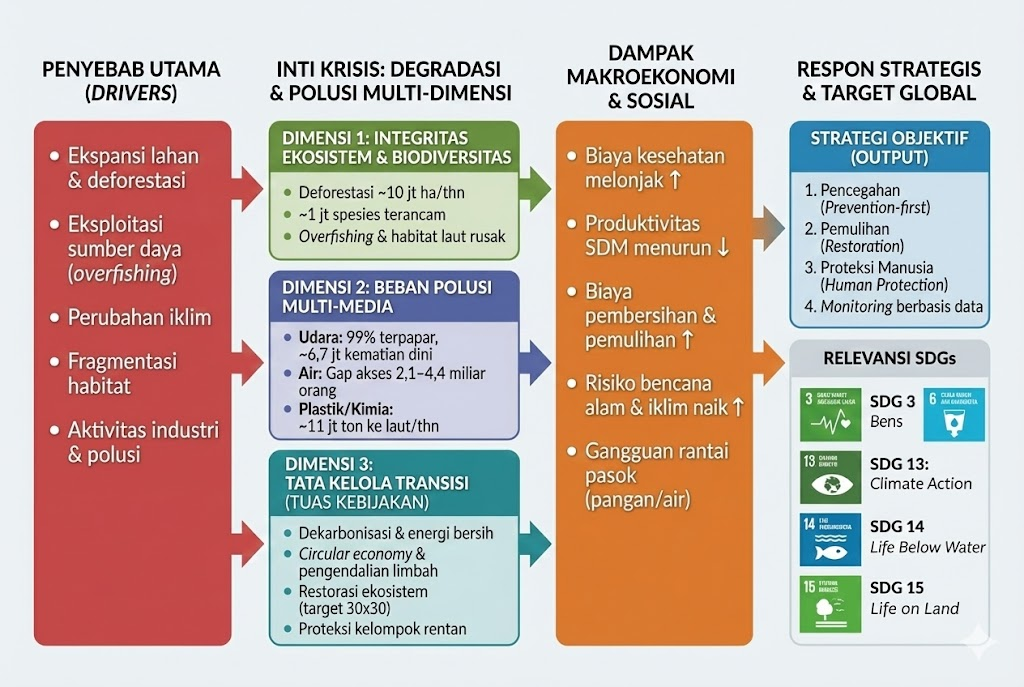
\includegraphics[width=1\linewidth,height=\textheight,keepaspectratio]{My_Concepts/./flowchart-lingkungan.jpg}

Konsep ``Degradasi Lingkungan dan Polusi'' menganalisis krisis
lingkungan global sebagai sistem yang saling terhubung, bukan isu
terpisah. Struktur konseptual ini membagi tantangan menjadi tiga dimensi
utama:

\begin{itemize}
\tightlist
\item
  \textbf{Integritas Ekosistem \& Keanekaragaman Hayati} --- kerusakan
  penopang kehidupan (hutan, laut, tanah, biodiversitas)
\item
  \textbf{Beban Polusi Multi-Media} --- pencemaran udara, air, dan tanah
  (termasuk plastik \& bahan kimia beracun)
\item
  \textbf{Tata Kelola Transisi \& Resiliensi} --- kapasitas kebijakan
  untuk menekan emisi/polusi, memulihkan ekosistem, dan melindungi
  populasi rentan
\end{itemize}

\subsection{Dimensi Integritas Ekosistem \& Keanekaragaman
Hayati}\label{dimensi-integritas-ekosistem-keanekaragaman-hayati}

\textbf{Warning --- Kerusakan Penopang Kehidupan}\\
Dimensi pertama membahas degradasi ekosistem yang mengurangi ``jasa
alam'' seperti penyediaan oksigen, penyerapan karbon, penyangga banjir,
dan sumber pangan.

\subsubsection{Data dan Fakta Kunci}\label{data-dan-fakta-kunci}

\begin{itemize}
\item
  Deforestasi global (2015--2020): \textasciitilde10 juta hektare per
  tahun.\\
  FAOHome
\item
  \textasciitilde1 juta spesies diperkirakan terancam punah (banyak
  ``dalam beberapa dekade'') akibat tekanan manusia.\\
  IPBES
\item
  Kerusakan ekosistem laut juga dipacu oleh eksploitasi berlebih dan
  degradasi habitat (contoh: stok ikan tidak berkelanjutan/overfished
  masih menjadi perhatian global).\\
  Reuters
\end{itemize}

\subsubsection{Faktor Penyebab (Driver)}\label{faktor-penyebab-driver}

\begin{itemize}
\tightlist
\item
  Ekspansi lahan (pertanian/perkebunan), pembalakan, kebakaran hutan
\item
  Perusakan habitat \& fragmentasi wilayah alami
\item
  Eksploitasi sumber daya berlebih (mis. penangkapan ikan)
\item
  Perubahan iklim (mempercepat tekanan ekosistem)
\item
  Polusi (memperburuk kualitas tanah, air, dan rantai makanan)
\end{itemize}

\textbf{Important}\\
Jika integritas ekosistem runtuh, biaya ekonomi meningkat melalui
hilangnya produktivitas, kerusakan aset, ketidakstabilan pangan/air, dan
risiko bencana yang lebih sering.

\subsection{Dimensi Beban Polusi
Multi-Media}\label{dimensi-beban-polusi-multi-media}

\textbf{Warning --- Polusi sebagai Krisis Kesehatan Publik \& Ekonomi}\\
Dimensi kedua menekankan bahwa polusi bukan sekadar ``isu lingkungan'',
tetapi risiko kesehatan terbesar dan penggerak biaya sosial--ekonomi.

\subsubsection{Polusi Udara (Ambient +
Household)}\label{polusi-udara-ambient-household}

\begin{itemize}
\item
  WHO melaporkan 99\% populasi global menghirup udara yang melampaui
  ambang pedoman WHO.\\
  World Health Organization
\item
  Dampak mortalitas: gabungan polusi udara luar-ruang dan rumah tangga
  terkait \textasciitilde6,7 juta kematian dini per tahun.\\
  World Health Organization
\end{itemize}

\subsubsection{Polusi Air (Minum \&
Paparan)}\label{polusi-air-minum-paparan}

\begin{itemize}
\item
  Estimasi resmi pemantauan global (WHO/UNICEF): sekitar 2,1 miliar
  orang masih tidak memiliki akses ``safely managed drinking water''.\\
  World Health Organization
\item
  Studi di Science (2024) menunjukkan estimasi bisa lebih besar:
  \textasciitilde4,4 miliar orang di LMICs diperkirakan kekurangan
  layanan air minum ``safely managed'' (terutama karena kontaminasi
  fekal dan akses).\\
  Science
\end{itemize}

Catatan konsep: Perbedaan angka ini penting untuk analisis
kebijakan---bukan kontradiksi sederhana, tetapi menunjukkan gap data \&
metode pengukuran.

\subsubsection{Polusi Tanah, Plastik, dan Bahan
Kimia}\label{polusi-tanah-plastik-dan-bahan-kimia}

\begin{itemize}
\item
  UNEP mengestimasi \textasciitilde11 juta ton plastik masuk ke laut
  setiap tahun (tanpa aksi, berisiko meningkat).\\
  UNEP - UN Environment Programme
\item
  Polutan kimia (mis. merkuri) berdampak langsung pada kesehatan dan
  ekosistem; respons global mencakup perjanjian seperti Minamata
  Convention.\\
  Minamata Convention
\end{itemize}

\subsubsection{Dampak Makroekonomi}\label{dampak-makroekonomi}

Polusi memicu:

\begin{itemize}
\tightlist
\item
  Biaya kesehatan naik (penyakit pernapasan/kardiovaskular, kanker,
  dll.)
\item
  Penurunan produktivitas tenaga kerja dan kualitas SDM
\item
  Biaya mitigasi \& pembersihan lingkungan
\item
  Gangguan rantai pasok (air bersih, pangan, energi) dan meningkatnya
  risiko bencana iklim
\end{itemize}

\subsection{Dimensi Tata Kelola Transisi \&
Resiliensi}\label{dimensi-tata-kelola-transisi-resiliensi}

\textbf{Warning --- Kapasitas Negara Menentukan ``Trajektori'' Krisis}\\
Dimensi ketiga mengukur kemampuan sistem (negara/kota/komunitas) untuk
mengubah lintasan degradasi lewat regulasi, insentif ekonomi, dan
perlindungan sosial.

\subsubsection{Tuas Kebijakan Kunci}\label{tuas-kebijakan-kunci}

\begin{itemize}
\tightlist
\item
  Dekarbonisasi energi \& transportasi (menekan polusi udara + emisi
  GRK)
\item
  Pengendalian limbah industri/pertanian (air \& tanah) + peningkatan
  IPAL
\item
  Circular economy: pengurangan plastik sekali pakai, desain ulang
  kemasan, EPR (extended producer responsibility)
\item
  Konservasi \& restorasi: perlindungan kawasan bernilai biodiversitas
  tinggi, rehabilitasi hutan/mangrove/DAS
\item
  Perlindungan kelompok rentan: adaptasi bencana, akses air bersih,
  peringatan dini, layanan kesehatan
\end{itemize}

\subsubsection{Indikator Tata Kelola (contoh
metrik)}\label{indikator-tata-kelola-contoh-metrik}

\begin{itemize}
\tightlist
\item
  Standar \& pemantauan kualitas udara (PM2.5, NO₂) + kepatuhan emisi
\item
  Cakupan layanan air minum aman \& uji kualitas mikrobiologi/kimia
\item
  Laju deforestasi \& luas restorasi tahunan
\item
  Tingkat kebocoran sampah plastik ke ekosistem per tahun
\item
  Proporsi kawasan lindung efektif (mis. arah kebijakan ``30x30''
  melindungi 30\% daratan \& lautan pada 2030)\\
  UNEP - UN Environment Programme
\end{itemize}

\subsection{Sintesis dan Indikator
Pencapaian}\label{sintesis-dan-indikator-pencapaian}

\subsubsection{Keterkaitan SDGs}\label{keterkaitan-sdgs}

\begin{itemize}
\tightlist
\item
  SDG 13 (Climate Action) --- emisi \& ketahanan bencana
\item
  SDG 14 (Life Below Water) --- sampah plastik, ekosistem laut,
  perikanan
\item
  SDG 15 (Life on Land) --- deforestasi, habitat, biodiversitas
\item
  SDG 3.9 --- pengurangan kematian/penyakit akibat polusi\\
  World Health Organization
\item
  SDG 6.1 --- akses air minum aman
\end{itemize}

\subsubsection{Data kunci krisis lingkungan
global}\label{data-kunci-krisis-lingkungan-global}

\begin{longtable}[]{@{}
  >{\raggedright\arraybackslash}p{(\linewidth - 4\tabcolsep) * \real{0.3000}}
  >{\raggedleft\arraybackslash}p{(\linewidth - 4\tabcolsep) * \real{0.4000}}
  >{\raggedright\arraybackslash}p{(\linewidth - 4\tabcolsep) * \real{0.3000}}@{}}
\toprule\noalign{}
\begin{minipage}[b]{\linewidth}\raggedright
Indikator
\end{minipage} & \begin{minipage}[b]{\linewidth}\raggedleft
Nilai (global)
\end{minipage} & \begin{minipage}[b]{\linewidth}\raggedright
Catatan
\end{minipage} \\
\midrule\noalign{}
\endhead
\bottomrule\noalign{}
\endlastfoot
Paparan udara tercemar & \textasciitilde99\% populasi & Di atas pedoman
WHO \nWorld Health Organization \n \\
Kematian dini terkait polusi udara & \textasciitilde6,7 juta/tahun &
Ambient + household \nWorld Health Organization \n \\
Kekurangan air minum ``safely managed'' (JMP) & \textasciitilde2,1
miliar orang & Estimasi pemantauan global \nWorld Health Organization
\n \\
Estimasi alternatif layanan air aman (Science 2024, LMICs) &
\textasciitilde4,4 miliar orang & Mengindikasikan gap data/metode
\nScience \n \\
Deforestasi & \textasciitilde10 juta ha/tahun (2015--2020) & Estimasi
FAO \nFAOHome \n \\
Plastik ke laut & \textasciitilde11 juta ton/tahun & Estimasi UNEP
\nUNEP - UN Environment Programme \n \\
Spesies terancam & \textasciitilde1 juta spesies & Estimasi IPBES
\nIPBES \n \\
\end{longtable}

\subsection{Strategi Objektif}\label{strategi-objektif}

Untuk menekan degradasi lingkungan dan polusi secara sistemik,
diperlukan integrasi tiga dimensi melalui:

\begin{itemize}
\tightlist
\item
  Pencegahan (prevention-first): standar emisi/limbah, energi bersih,
  transport publik, tata kelola sampah
\item
  Pemulihan (restoration): restorasi hutan/DAS, rehabilitasi pesisir \&
  ekosistem kritis
\item
  Proteksi manusia (human protection): air bersih, layanan kesehatan,
  adaptasi bencana, jaring pengaman sosial
\item
  Monitoring berbasis data: sensor kualitas udara, uji air, audit
  limbah, pelaporan transparan
\end{itemize}

\textbf{Tip --- Kesimpulan}\\
Jika integritas ekosistem terjaga, polusi ditekan, dan tata kelola
transisi kuat, negara akan memperoleh ``dividen'' makro: kesehatan
meningkat, produktivitas naik, risiko bencana turun, dan pertumbuhan
ekonomi lebih stabil serta inklusif.

\bookmarksetup{startatroot}

\chapter{UAS-3 My Opinions}\label{uas-3-my-opinions}

\bookmarksetup{startatroot}

\chapter{7 UAS-3 My Opinions}\label{uas-3-my-opinions-1}

\section{7.1 Rekonstruksi Ketahanan Lingkungan melalui Strategi
``ECO-SHIELD''}\label{rekonstruksi-ketahanan-lingkungan-melalui-strategi-eco-shield}

\begin{tcolorbox}[enhanced jigsaw, toprule=.15mm, arc=.35mm, colframe=quarto-callout-note-color-frame, left=2mm, titlerule=0mm, title=\textcolor{quarto-callout-note-color}{\faInfo}\hspace{0.5em}{Posisi Opini}, leftrule=.75mm, colbacktitle=quarto-callout-note-color!10!white, toptitle=1mm, bottomrule=.15mm, opacitybacktitle=0.6, breakable, coltitle=black, colback=white, opacityback=0, bottomtitle=1mm, rightrule=.15mm]

Opini ini menyoroti perlunya \textbf{pergeseran paradigma}: degradasi
lingkungan dan polusi harus diperlakukan sebagai \textbf{krisis
sistemik} (ekosistem + polusi + tata kelola), bukan sekadar proyek
terpisah seperti ``tanam pohon sekali'', ``bersih-bersih pantai'', atau
``kampanye hemat listrik'' tanpa desain kebijakan yang menyatu.

\end{tcolorbox}

\subsection{7.1.1 Konteks Kegagalan
Sistemik}\label{konteks-kegagalan-sistemik}

Pendekatan konvensional yang hanya fokus pada \textbf{aksi parsial}
(mis. program satu sektor, satu wilayah, satu tahun) terbukti
\textbf{belum mampu menyelesaikan masalah}, karena sumber masalahnya
lintas-sektor dan saling menguatkan:

\begin{itemize}
\tightlist
\item
  \textbf{\textasciitilde10 juta ha/tahun} deforestasi global
  (2015--2020) → melemahkan penyerapan karbon \& meningkatkan risiko
  banjir/kekeringan\\
\item
  \textbf{\textasciitilde1 juta spesies} diperkirakan terancam punah →
  jaringan penyangga ekosistem runtuh\\
\item
  \textbf{99\% populasi} global menghirup udara melebihi pedoman WHO →
  paparan hampir universal\\
\item
  \textbf{\textasciitilde6,7 juta} kematian dini/tahun terkait polusi
  udara (gabungan ambient + household)\\
\item
  \textbf{2,1--4,4 miliar} orang mengalami gap akses air minum aman
  (beda estimasi mengindikasikan gap data \& metode)\\
\item
  \textbf{\textasciitilde11 juta ton/tahun} sampah plastik masuk ke laut
  → merusak rantai makanan \& ekosistem pesisir
\end{itemize}

\section{Kebutuhan Model Baru}\label{kebutuhan-model-baru}

Diperlukan model yang mengintegrasikan \textbf{Drivers → Dimensi Krisis
→ Dampak → Strategi} secara konsisten, dengan indikator yang bisa
dipantau (udara, air, deforestasi, kebocoran plastik, dan target
perlindungan 30x30).

\subsection{7.1.2 Strategi ``ECO-SHIELD'' (Kerangka
Solusi)}\label{strategi-eco-shield-kerangka-solusi}

Saya mengusulkan strategi \textbf{ECO-SHIELD} sebagai kerangka yang
menyatukan 3 dimensi krisis:

\begin{enumerate}
\def\labelenumi{\arabic{enumi}.}
\item
  \textbf{Ecosystem Integrity}\\
  Menahan laju kerusakan ekosistem (hutan, laut, tanah) + restorasi area
  kritis.
\item
  \textbf{Pollution Control (Multi-media)}\\
  Menekan polusi \textbf{udara--air--tanah} sekaligus (bukan hanya satu
  media).
\item
  \textbf{Governance \& Resilience}\\
  Menguatkan tata kelola transisi: regulasi, insentif ekonomi,
  perlindungan kelompok rentan, dan respons bencana.
\end{enumerate}

\subsection{7.1.3 Dampak Makroekonomi \& Sosial (Kenapa Ini Bukan ``Isu
Alam''
Saja)}\label{dampak-makroekonomi-sosial-kenapa-ini-bukan-isu-alam-saja}

Jika krisis dibiarkan, jalurnya jelas:

\begin{itemize}
\tightlist
\item
  \textbf{Biaya kesehatan meningkat} (penyakit
  pernapasan/kardiovaskular, dll.)
\item
  \textbf{Produktivitas SDM menurun} → pendapatan dan daya saing turun
\item
  \textbf{Biaya pemulihan \& pembersihan} naik
\item
  \textbf{Risiko bencana} (banjir, kekeringan) meningkat
\item
  \textbf{Gangguan rantai pasok} (pangan/air/energi) makin sering
\end{itemize}

\subsection{7.1.4 Output: Respon Strategis (yang harus
dilakukan)}\label{output-respon-strategis-yang-harus-dilakukan}

\begin{enumerate}
\def\labelenumi{\arabic{enumi}.}
\item
  \textbf{Pencegahan (prevention-first)}\\
  Standar emisi \& transport publik, kontrol limbah industri/pertanian,
  pengurangan plastik sekali pakai + EPR.
\item
  \textbf{Pemulihan (restoration)}\\
  Restorasi hutan/DAS, rehabilitasi pesisir \& ekosistem kritis
  (mangrove/terumbu).
\item
  \textbf{Proteksi manusia (human protection)}\\
  Air minum aman, layanan kesehatan, adaptasi bencana \& jaring pengaman
  sosial untuk kelompok rentan.
\item
  \textbf{Monitoring berbasis data}\\
  Sensor PM2.5, uji kualitas air, audit limbah, pelaporan transparan
  untuk evaluasi kebijakan.
\end{enumerate}

\subsection{7.1.5 Relevansi Target Global
(SDGs)}\label{relevansi-target-global-sdgs}

\begin{itemize}
\tightlist
\item
  \textbf{SDG 13} (Climate Action)\\
\item
  \textbf{SDG 14} (Life Below Water)\\
\item
  \textbf{SDG 15} (Life on Land)\\
\item
  \textbf{SDG 3.9} (mengurangi kematian/penyakit akibat polusi)\\
\item
  \textbf{SDG 6.1} (akses air minum aman)
\end{itemize}

\begin{tcolorbox}[enhanced jigsaw, toprule=.15mm, arc=.35mm, colframe=quarto-callout-tip-color-frame, left=2mm, titlerule=0mm, title=\textcolor{quarto-callout-tip-color}{\faLightbulb}\hspace{0.5em}{Kesimpulan}, leftrule=.75mm, colbacktitle=quarto-callout-tip-color!10!white, toptitle=1mm, bottomrule=.15mm, opacitybacktitle=0.6, breakable, coltitle=black, colback=white, opacityback=0, bottomtitle=1mm, rightrule=.15mm]

Ketahanan lingkungan bukan ``bonus moral'', tapi \textbf{fondasi
ekonomi}. Jika ekosistem dijaga, polusi ditekan, dan tata kelola
transisi kuat, negara memperoleh ``dividen'' makro: \textbf{kesehatan
naik, produktivitas naik, risiko bencana turun, ekonomi lebih stabil dan
inklusif}.

\end{tcolorbox}

\bookmarksetup{startatroot}

\chapter{UAS-3 My Innovations}\label{uas-3-my-innovations}

\bookmarksetup{startatroot}

\chapter{UAS-4 My Knowledge}\label{uas-4-my-knowledge}

Cara saya mengkomunikasikan sebuah pengatahuan sebagai petunjuk bagi
orang lain 1) saya tulis
\href{Rekomendasi\%20Presentasi\%20Efektif(Contoh\%20Makalah).pdf}{makalah
sebagai bahan utama} 2) lalu saya buat
\href{Contoh\%20Transkrip\%20Presentasi.pdf}{transkrip ucapan lisan} 3)
kemudian saya kembangkan
\href{Rekomendasi\%20Presentasi\%20(Contoh\%20Slides).pdf}{slide
pendukung trnsskrip} 4) lalu saya memproduksivideo audio visual
\url{https://youtu.be/ZbghfMvnPZc} \url{https://youtu.be/ZbghfMvnPZc}

\bookmarksetup{startatroot}

\chapter{UAS-5 My Professional
Reviews}\label{uas-5-my-professional-reviews}

Untuk melAkukan review, seperti pada
\href{../My_Personal_Reviews/Doc.5.Mengevaluasi-Esai-Berdasarkan-Rubrik.pdf}{pendekatan
AI}, kita membutuhkan rubrik

\bookmarksetup{startatroot}

\chapter{Summary}\label{summary}

In summary, this book has no content whatsoever.

\bookmarksetup{startatroot}

\chapter*{References}\label{references}
\addcontentsline{toc}{chapter}{References}

\markboth{References}{References}

\phantomsection\label{refs}




\end{document}
